For each of the three tasks, we first assess the
performance of our base model to (1) verify our sampling-based
Bayesian implementations, and (2) compare to the state of the art.  We train each
model with a Metropolis-within-Gibbs sampler with 50,000 samples using
PyMC~\cite{Patil:2010,Salvatier:2015}, discarding the first half of the samples
as burn-in.  The variances $m_{\sigma_w}$ and $m_{\sigma_S}$ are both set to
100.  Base models are evaluated on the entire test set for each task, and the
same training examples as in the state-of-the-art systems are used.
\Cref{table:base-models-results} shows the results.

Following SemEval, we report a weighted sum of correlations (Pearson's
$r$) across all test sets for \sts{}, where the weight of a test set
is proportional to its number of pairs.  Our model and
\newcite{Sultan:2015} are almost identical on all twenty test sets
from SemEval 2012--2015, supporting the correctness of our Bayesian
implementation.

\begin{table}[t]
\centering
\small
\begin{tabular}{c|c|c}
\hline
\hline
\textbf{Task} & \textbf{Current SOA} & \textbf{Our Model} \\
\hline
\hline
\sts{} & Pearson's $r$ = 73.6\% & Pearson's $r$ = 73.7\% \\
\hline
\multirow{2}{*}{\sas{}} & Pearson's $r$ = 51.8\% & Pearson's $r$ = 56.4\% \\
                     & \abr{rmse} = 19.6\% & \abr{rmse} = 18.1\% \\
\hline
\multirow{2}{*}{\asr{}} & \abr{map} = 74.6\% & \abr{map} = 76.0\% \\
                     & \abr{mrr} = 80.8\% & \abr{mrr} = 82.8\% \\
\hline
\hline
\end{tabular}
\caption{
Our base linear models beat the state of the art in
\sts{}, \sas{} and \asr{}.
}
\label{table:base-models-results}
\end{table}

Following \newcite{Mohler:2011}, for \sas{} we use \abr{rmse}
and Pearson's $r$ with gold scores over all answers.
These metrics are complementary: correlation is a measure of
consistency across students while error measures deviation from
individual scores.  Our model beats the state-of-the-art text
matching model of \newcite{Mohler:2011} on both
metrics.\footnote{\newcite{Ramachandran:2015} report better results;
  however, they evaluate on a much smaller random subset of the test
  data and use in-domain annotations for model training.}

Finally, for \asr{}, we adopt two metrics widely used in information
retrieval: mean average precision (\abr{map}) and mean reciprocal rank
(\abr{mrr}).  \abr{map} assesses the quality of the ranking as a whole whereas
\abr{mrr} evaluates only the top-ranked answer sentence.  \newcite{Severyn:2015}
report a convolutional neural network model of text similarity which shows top
\asr{} results on the \newcite{Wang:2007} dataset.  Our model outperforms
this model on both metrics.

\subsection{Adaptation to \sts{} Domains}
\label{section:experiments-sts-da}


Ideally, our domain adaptation (\da{}) should allow the application of
large amounts of out-of-domain training data along with few in-domain
examples to improve in-domain performance.  Given data from $n$
domains, two other alternatives in such scenarios are: (1) to train a
single \emph{global} model using all available training examples, and
(2) to train $n$ \emph{individual} models, one for each domain, using
only in-domain examples.  \Cref{section:tasks-and-datasets-sts} shows
results from our \da{} model and these two baselines on the ten \sts{}
datasets.  We fix the training set size and split each
domain into train and test folds randomly.

Models have access to training data from all ten domains (thus nine times more
out-of-domain examples than in-domain ones).  Each model (global, individual,
and adaptive) is trained on relevant annotations and applied to test pairs,
and Pearson's $r$ with gold scores is computed for each model on each individual
test set.  Since performance can vary across different splits, we average over
20 splits of the same train/test ratio per dataset.  Finally, we evaluate each
model with a weighted sum of average correlations across all test sets, where
the weight of a test set is proportional to its number of pairs.

\begin{figure}[t]
\centering
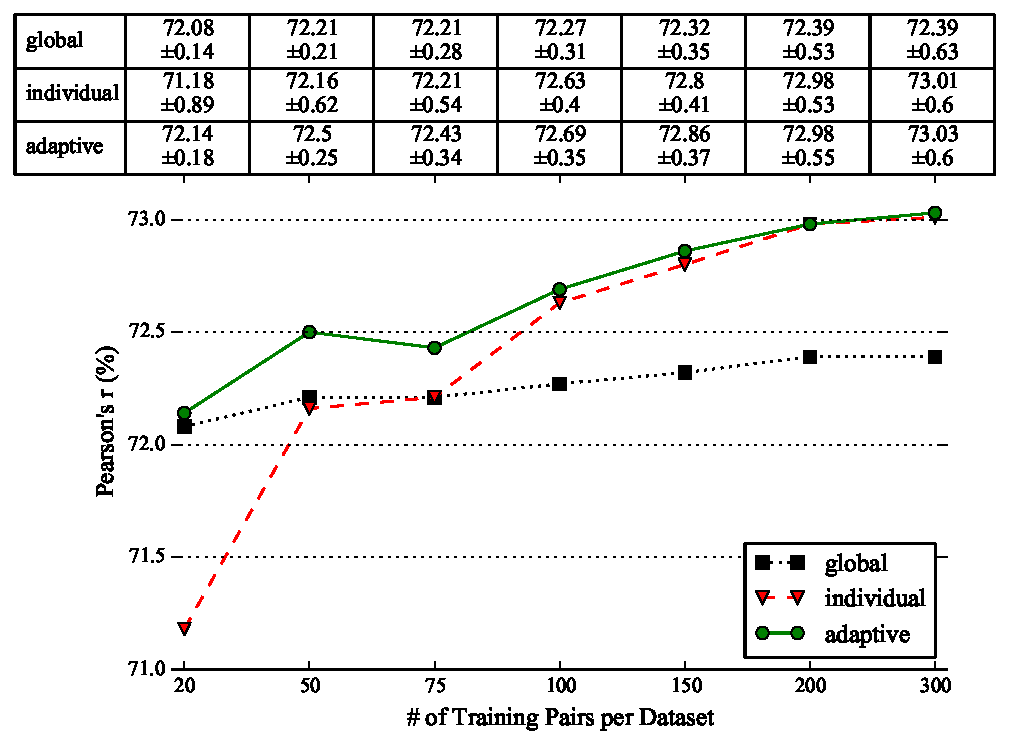
\includegraphics[scale=0.47]{2016_naacl_stsdomain/figures/sts_da_results.pdf}
\caption{
	Results of adaptation to \sts{} domains across
	different amounts of training data.
	Table shows mean$\pm$SD from 20 random train/test splits.
    While the baselines falter at extremes,
    the adaptive model shows consistent performance.
}
\label{figure:sts-da-results}
\end{figure}


\Cref{figure:sts-da-results} shows how models adapt as the training set grows.


The global model clearly falters with larger training sets in
comparison to the other two models.  On the other hand, the
domain-specific model (i.e., the ten individual models) performs
poorly when in-domain annotations are scarce.  Importantly, the
adaptive model performs well across different amounts of available
training data.

To gain a deeper understanding of model performance, we examine results in
individual domains.  A single performance score is computed for every model-domain pair
by taking the model's average correlation in that domain over all seven training set
sizes of \Cref{figure:sts-da-results}.
We then normalize each score by dividing by the best score in that domain.  Each cell
in \Cref{table:sts-results-on-individual-domains} shows this score for a
model-domain pair.  For example, Row~1 shows that---on average---the individual
model performs the best (hence a correlation ratio of 1.0) on \qa{} forum answer pairs
while the global model performs the worst.

\begin{table}[t]
\centering
\small
\begin{tabular}{l|c|c|c}
\hline
\hline
\multicolumn{1}{c|}{\textbf{Dataset}} & \textbf{Glob.} & \textbf{Indiv.} & \textbf{Adapt.} \\
\hline
\hline
Answers-forums (2015) & \underline{.9847} & \textbf{1} & .9999 \\

Answers-students (2015) & \underline{.9850} & \textbf{1} & .9983 \\

Belief (2015) & \textbf{1} & \underline{.9915} & .9970 \\

Headlines (2015) & \underline{.9971} & .9998 & \textbf{1} \\

Images (2015) & .9992 & \underline{.9986} & \textbf{1} \\

Deft-forum (2014) & \textbf{1} & \underline{.9775} & .9943 \\

On\abr{wn} (2014) & \underline{.9946} & .9990 & \textbf{1} \\

Tweet-news (2014) & .9998 & \underline{.9950} & \textbf{1} \\

\abr{smt} (2013) & \textbf{1} & \underline{.9483} & .9816 \\

\abr{msr}par-test (2012) & \underline{.9615} & \textbf{1} & .9923 \\

\hline
\multicolumn{1}{c|}{Mean} & .9918 & \underline{.9911} & \textbf{.9962} \\

\multicolumn{1}{c|}{SD} & .0122 & .0165 & .0059 \\
\hline
\hline
\end{tabular}
\caption{
  Correlation ratios of the three models vs. the best model across \sts{}
  domains.  Best scores are
  \textbf{boldfaced}, worst scores are \underline{underlined}.
  The adaptive model has the best (1) overall score, and (2) consistency
  across domains.
}
\label{table:sts-results-on-individual-domains}
\end{table}



While the adaptive model is not the best in every domain, it has the
best worst-case performance across domains.  The global model suffers
in domains that have unique parameter distributions
(e.g., \abr{msr}par-test: a paraphrase dataset).  The individual model
performs poorly with few training examples and in domains with noisy
annotations (e.g., \abr{smt}: a machine translation evaluation
dataset).  The adaptive model is much less affected in such extreme
cases.  The summary statistics (weighted by dataset size) confirm that
it not only stays the closest to the best model on average, but also
deviates the least from its mean performance level.

\begin{table}[t]
\centering
\small
\begin{tabular}{l|c|c|c|c}
\hline
\hline
\multicolumn{1}{c|}{\textbf{Dataset}} & \textbf{Var.} & \textbf{Glob.} & \textbf{Indiv.} & \textbf{Adapt.} \\

\hline
\hline
\multirow{3}{*}{\abr{smt}} & $w_1$ & .577 & .214 & .195 \\
& $w_2$ & .406 & -.034 & .134 \\
\cline{2-5}
& $r$ & \textbf{.4071} & .3866 & \textbf{.4071} \\
\hline
\multirow{3}{*}{\abr{msr}par-test} & $w_1$ & .577 & 1.0 & .797 \\
& $w_2$ & .406 & -.378 & .050 \\
\cline{2-5}
& $r$ & .6178 & \textbf{.6542} & .6469 \\
\hline
\multirow{3}{*}{Answers-students} & $w_1$ & .577 & .947 & .865 \\
& $w_2$ & .406 & .073 & .047 \\
\cline{2-5}
& $r$ & .7677 & \textbf{.7865} & .7844 \\



\hline
\hline
\end{tabular}
\caption{
  Feature weights and correlations of different models in three extreme scenarios.
  In each case, the adaptive model learns relative weights that are more similar
  to those in the best baseline model.
}
\label{table:sts-da-weights}
\end{table}

\subsubsection{Qualitative Analysis}


We further examine the models to understand \emph{why} the
adaptive model performs well in different extreme scenarios, i.e., when one
of the two baseline models performs worse than the other.
\Cref{table:sts-da-weights} shows feature weights learned by each model from
a split with seventy-five training pairs per domain and how well each
model does.

All three domains have very different outcomes for the baseline models.  We show weights for the
alignment ($w_1$) and embedding features ($w_2$).  In each domain,
(1) the relative weights learned by the two baseline models are very
different, and (2) the adaptive model learns relative weights that are
closer to those of the best model.  In \abr{smt}, for example, the
predictor weights learned by the adaptive model have a ratio very
similar to the global model's and does just as well.
On Answers-students, however, it learns weights similar to those of
the in-domain model, again approaching best results for the domain.

\Cref{table:sentence-examples} shows the effect of this on two specific sentence
pairs as examples.  The first pair is from \abr{smt}; the adaptive model has a
much lower error than the individual model on this pair, as it learns a higher
relative weight for the embedding feature in this domain
(\Cref{table:sts-da-weights}) via inductive transfer from out-of-domain
annotations.  The second pair, from \abr{msr}par-test, shows the opposite:
in-domain annotations helps the adaptive model fix the faulty output of the
global model by upweighting the alignment feature and downweighting the
embedding feature.



The adaptive model gains from the strengths of both in-domain (higher
relevance) and out-of-domain (more training data) annotations, leading
to good results even in extreme scenarios (e.g., in domains with
unique parameter distributions or noisy annotations).


\begin{table}
\centering
\small

\begin{tabular}{p{.33\textwidth}|p{.08\textwidth}}
  \hline
  \hline
  Now, the labor of cleaning up at the karaoke parlor is realized. &
  				\multirow{4}{*}
  				{
  					\begin{minipage}{.09\textwidth}
	  					Gold=.52 $\Delta$G=\textbf{.1943} $\Delta$I=.2738 $\Delta$A=.2024
	  				\end{minipage}
	  			} \\
  \cline{1-1}
  Up till now on the location the cleaning work is already completed. &  \\

  \Xhline{2\arrayrulewidth}
  The Chelsea defender Marcel Desailly has been the latest to speak out. &
			    \multirow{5}{*}
  				{
  					\begin{minipage}{.09\textwidth}
	  					Gold=.45 $\Delta$G=.2513 $\Delta$I=\textbf{.2222} $\Delta$A=.2245
	  				\end{minipage}
	  			} \\
  \cline{1-1}
  Marcel Desailly, the France captain and Chelsea defender, believes the latter is true. & \\
  \hline
  \hline

\end{tabular}
\caption{
Sentence pairs from \abr{smt} and \abr{msr}par-test with gold similarity scores
and model errors (\underline{G}lobal, \underline{I}ndividual
and \underline{A}daptive). The adaptive model error is very close to the
best model error in each case.
}
\label{table:sentence-examples}
\end{table}



\subsection{Multitask Learning}


We now analyze performance of our multitask learning (\mtl{}) model in
each of the three tasks:
\sts{}, \sas{} and \asr{}.  Multitaks baselines resemble \da{}'s:
 (1) a global model trained on all available training data
(\Cref{figure:sts-sas-asr-model}), and (2) nineteen task-specific
models, each trained on an individual dataset from one of the three
tasks (\Cref{figure:base-models}).  The smallest of these datasets has
only 204 pairs (\sas{} assignment \#1); therefore, we use training
sets with up to 175 pairs per dataset.  Because the \mtl{} model is
more complex, we use a stronger regularization for this model
($m_{\sigma_w}$=10) while keeping the number of \abr{mcmc} samples
unchanged.  As in the \da{} experiments, we compute average
performance over twenty random train/test splits for each training set
size.

\Cref{figure:sts-mtl-results} shows \sts{} results for all models across
different training set sizes.  Like \da{}, the adaptive model
consistently performs well while the global and individual models have
different failure modes.  However, the individual model does better
than in \da{}: it overtakes the global model with fewer training
examples and the differences with the adaptive model are smaller.
This suggests that inductive transfer and therefore adaptation is less
effective for \sts{} in the \mtl{} setup than in \da{}.
Later in this section, coarse-grained \asr{}
annotations (binary as opposed to real-valued) in \mtl{} may provide
an explanation for this.


The performance drop after 150 training pairs is a likely
consequence of the random train/test selection process.

\begin{figure}[t]
\centering
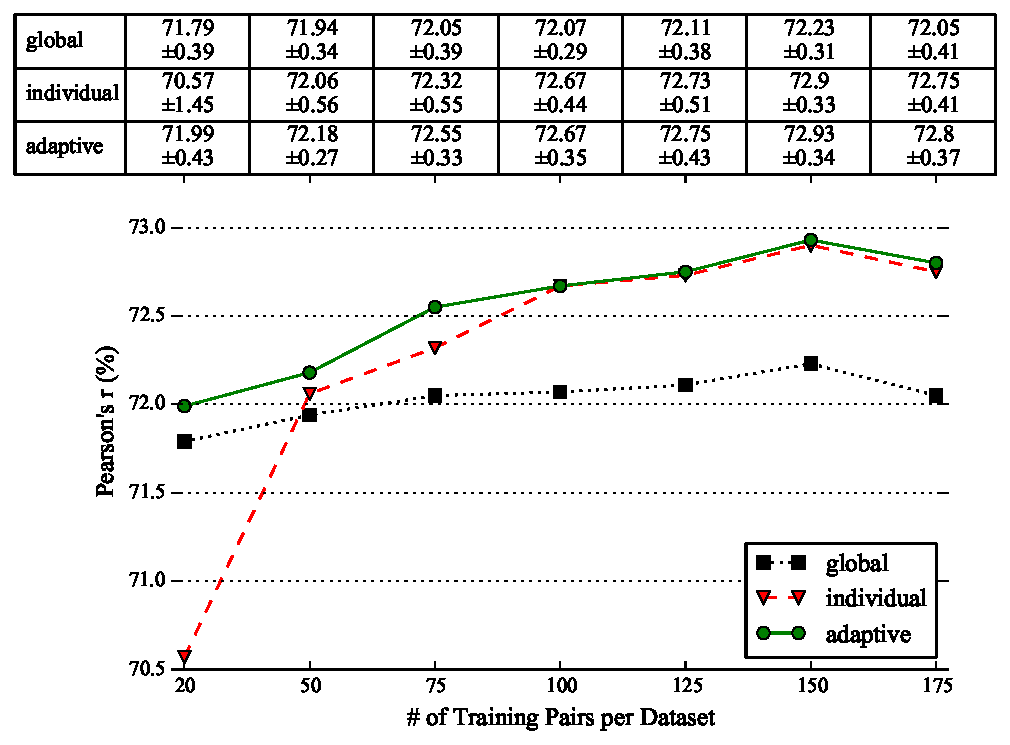
\includegraphics[scale=0.47]{2016_naacl_stsdomain/figures/sts_multitask_learning_results.pdf}
\caption
{Multitask learning for \sts{}: mean$\pm$\abr{sd} from
twenty random train/test splits.  The adaptive model consistently
performs well while the baselines have different failure modes.  }
\label{figure:sts-mtl-results}
\end{figure}

\begin{figure*}
    \begin{subfigure}[b]{0.5\textwidth}
        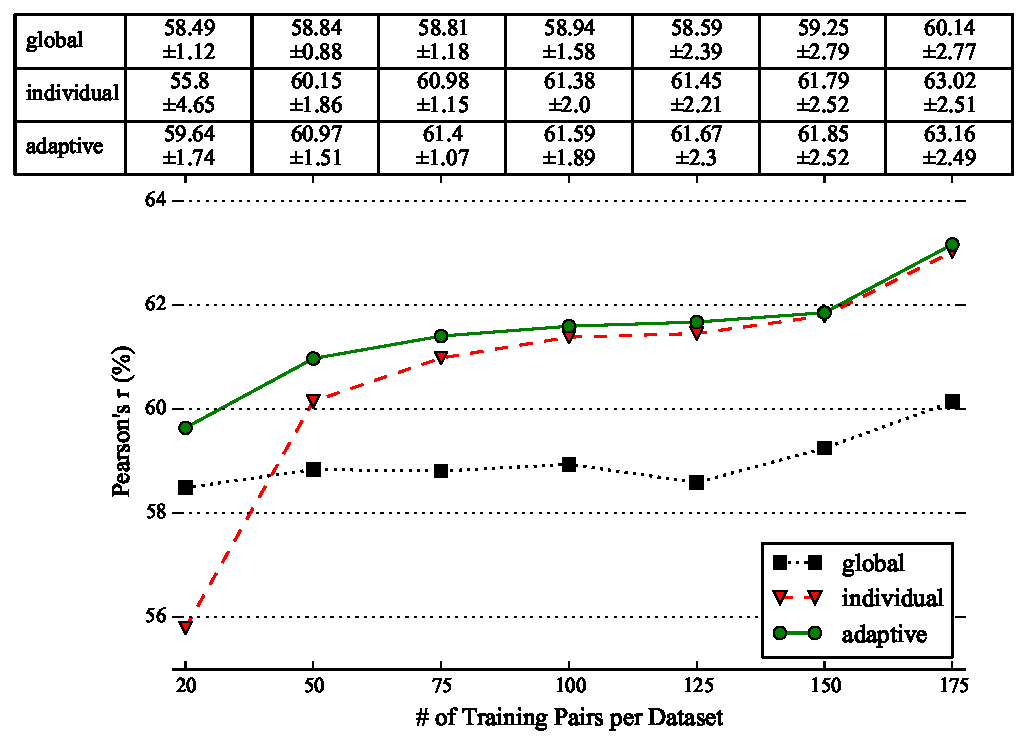
\includegraphics[scale=0.47]{2016_naacl_stsdomain/figures/sas_multitask_learning_correlations.pdf}
        \caption{Correlation.}
        \label{figure:sas-multitask-learning-correlations}
    \end{subfigure}
    \begin{subfigure}[b]{0.45\textwidth}
        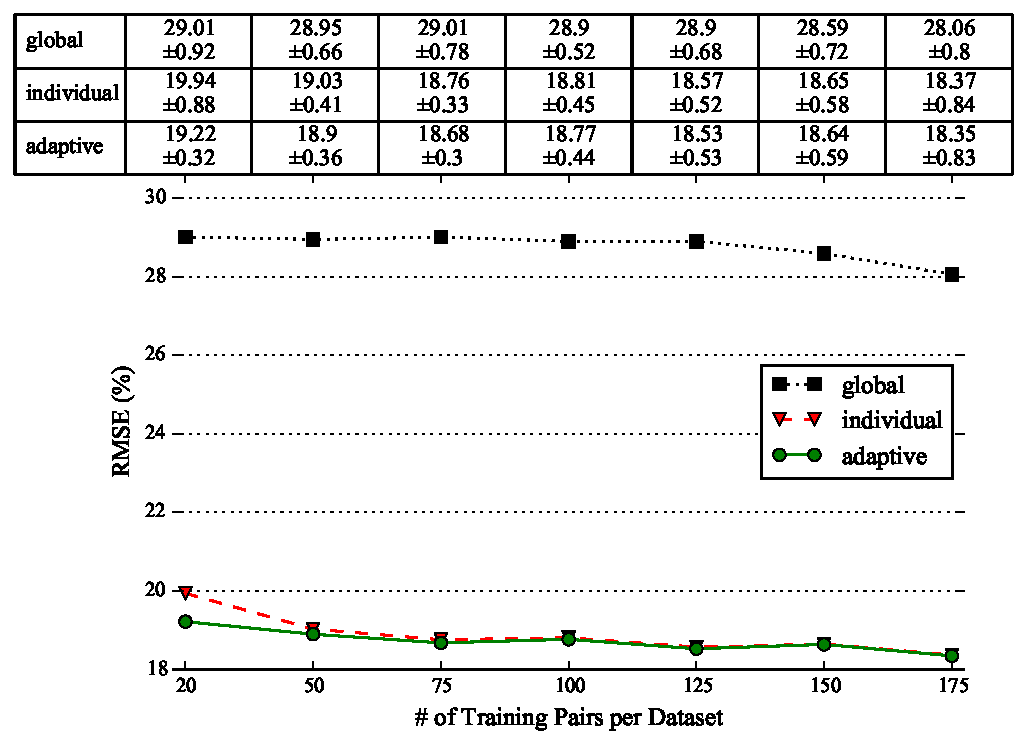
\includegraphics[scale=0.47]{2016_naacl_stsdomain/figures/sas_multitask_learning_rmses.pdf}
        \caption{Error.}
        \label{figure:sas-multitask-learning-errors}
    \end{subfigure}
    \newline
    \caption{Multitask learning for \sas{}: mean$\pm$SD from 20 random
    train/test splits.  The adaptive model performs the best, and
    successfully handles domain shift evident from the global model
    error.}
    \label{figure:sas-mtl-results}
\end{figure*}

\begin{figure*}
    \begin{subfigure}[b]{0.5\textwidth}
        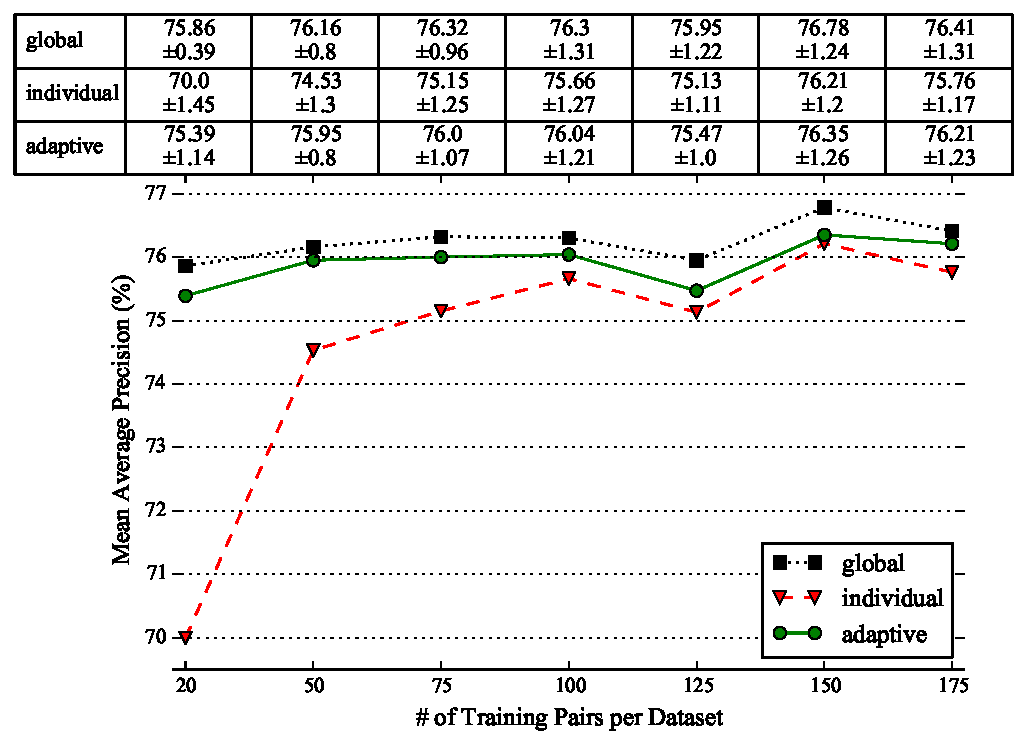
\includegraphics[scale=0.47]{2016_naacl_stsdomain/figures/asr_multitask_learning_maps.pdf}
        \caption{Mean Average Precision.}
        \label{figure:asr-multitask-learning-maps}
    \end{subfigure}
    
    
    \begin{subfigure}[b]{0.45\textwidth}
        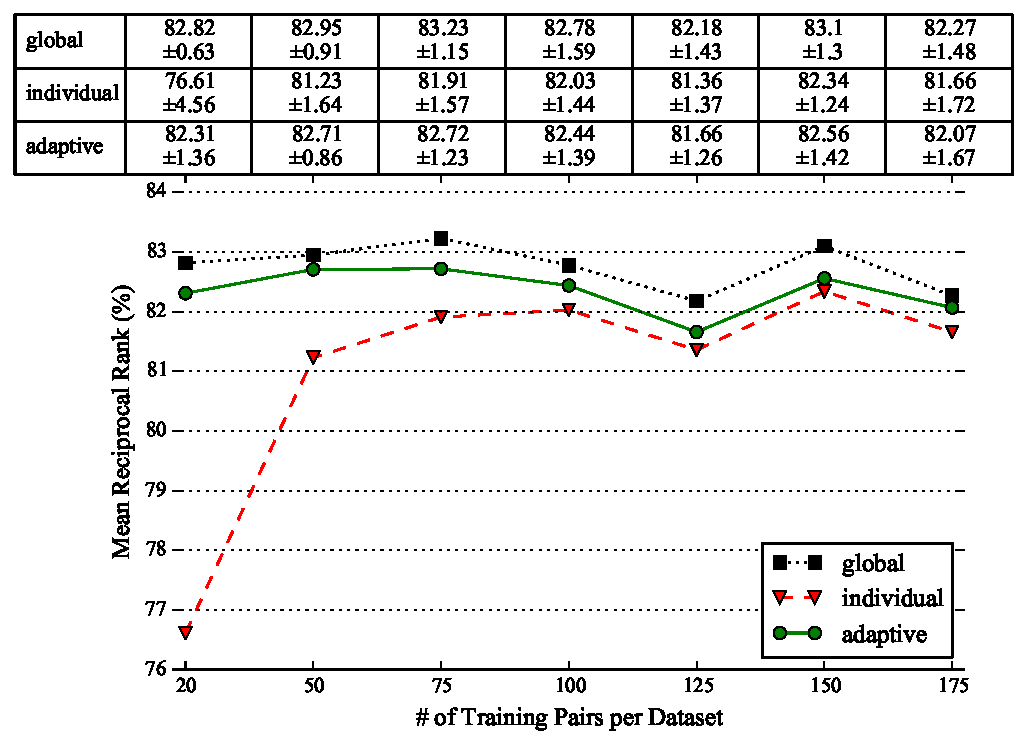
\includegraphics[scale=0.47]{2016_naacl_stsdomain/figures/asr_multitask_learning_mrrs.pdf}
        \caption{Mean Reciprocal Rank.}
        \label{figure:asr-multitask-learning-mrrs}
    \end{subfigure}
    \newline
    \caption{Multitask learning for \asr{}: mean$\pm$SD from 20 random train/test splits.
    Least affected by coarse-grained in-domain annotations, the
    global model performs the best; the adaptive model
    stays close across all training set sizes.}
    \label{figure:asr-mtl-results}
\end{figure*}



For \sas{}, the adaptive model again has the best overall performance for both
correlation and error (\Cref{figure:sas-mtl-results}).  The correlation plot is
qualitatively similar to the \sts{} plot, but the global model has a much higher
\abr{rmse} across all training set sizes, indicating a parameter shift across
tasks.  Importantly, the adaptive model remains unaffected by this shift.

The \asr{} results in \Cref{figure:asr-mtl-results} show a different pattern.
Contrary to all results thus far, the global model performs the best in this
task.  The individual model consistently has lower scores, regardless of the
amount of training data.  Importantly, the adaptive model stays close to the
global model even with very few training examples.  The \asr{} datasets are
heavily biased towards negative examples; thus, we use stratified sampling to
ensure each \asr{} training set has balanced examples.

A reason for the global model's strength at \asr{} may lie in
the finer granularity of the real-valued \sts{} and \sas{} scores compared to
binary \asr{} annotations.  If a fine granularity is indeed desirable in
training data, as a model that ignores in-domain and out-of-domain distinction, the
global model would be affected the least by coarse-grained \asr{} annotations.
To test this hypothesis, we train a linear model on all \sts{} examples from
SemEval 2012--2015 and apply it to the \asr{} test set via a logistic
transformation.  This model indeed demonstrates better results (\abr{map}=.766,
\abr{mrr}=.839) than our base model trained on \asr{} annotations
(\Cref{table:base-models-results}).  This is an unusual scenario where in-domain
training examples matter less than out-of-domain ones, hurting
domain-specific and adaptive models.

Going back to \sts{}, this finding also offers an explanation of why adaptation
might have been less useful in multitask learning than in domain adaptation,
as only the former has \asr{} annotations.
